

\section{Relic Density}
\label{sec:relic}

In the standard %Uli 
%Weakly Interacting Massive Particle (WIMP) 
% 
thermal relic ``freeze-out" picture of the early Universe,
the annihilation rate of DM particles into normal matter determines the temperature at which DM decouples from thermal equilibrium and sets the DM density observed today.
%Uli 
One can use the simplified models discussed in Section~\ref{sec:models} to predict the relic density and compare with measurements such as the most recent results by the Planck collaboration~\cite{Ade:2015xua} to gain insight on interesting regions of the model parameter space. In order to do so, one has to make the following assumptions:
\begin{itemize}
\item The DM annihilation cross section receives only contributions from the interactions of the simplified model, while possible additional degrees of freedom and couplings not included in the model are irrelevant. 
\item The DM number density in the Universe today is entirely determined by  the DM annihilation cross section predicted by the simplified model. In particular, no additional mechanisms exist that enhance or deplete the relic density.
\end{itemize}

It it important to realize that if one or both of these assumptions are violated there is no strict correlation between the relic density and the strength of mono-$X$ signals. For instance, if DM is overproduced, the relic density can be reduced if the DM has large annihilation cross sections to new hidden sector states. These states might however not be directly accessible at LHC energies.  Conversely, the correct DM relic density can still be obtained  if the DM is underproduced. For instance, if the hidden sector carries an particle-antiparticle asymmetry (similar to the baryon asymmetry) then this necessarily leads to a larger relic density compared to the conventional freeze-out picture. 

%In other words, if 
%\begin{itemize}
%\item DM couples to SM matter only through the one mediator explicitly included in the simplified model.
%\item The mediator has no other coupling (to SM or undiscovered particles) than those listed for each model in Section~\ref{sec:models}.
%\item No additional mechanisms exist to generate or deplete DM.
%\end{itemize}
%then one can use the simplified model to predict the relic density %and compare with measurements such as the most recent results by the Planck collaboration~\cite{Ade:2015xua} to gain insight on interesting regions of the model parameter space.

%Uli For the overall approach, consult Section 3.3.1 of an earlier document~\cite{Boveia:2016mrp} from this working group. When adding lepton couplings as above, the calculation changes, as it is now possible for DM particles to annihilate into pairs of charged leptons or neutrinos.

%Uli
In this section, we assume that the two aforementioned assumptions are satisfied, and  present an analytic calculation of the relic density for the dominant annihilation processes that involve spin-0 and spin-1 mediators. We then provide numerical computations of the relic density for the  scalar, pseudo-scalar, vector, and axial-vector simplified model scenarios using version 2.0 of the \dmsimp implementation~\cite{DMsimp}
%of the simplified model scenarios
%~\cite{Backovic:2015soa,Neubert:2015fka,Mattelaer:2015haa} 
and version 2.0.6 of \maddm~\cite{Backovic:2013dpa,Backovic:2015tpt}. The Lagrangians for these models can be found in~\cite{Boveia:2016mrp} and references therein. 

For concreteness  the coupling values recommended for the first Run-2 results by the ATLAS/CMS %Uli Dark Matter Forum 
DMF are used in this section. The couplings of the spin-1 mediator (vector or axial-vector) to SM quarks is chosen to be $g_q = 0.25$ and the lepton coupling value is set to zero, corresponding to scenarios V1 and A1 of Section~\ref{sub:vecAxial}. The coupling value of the spin-0 mediator (scalar or pseudo-scalar) to quarks is chosen to be $g_q=1.0$ with an implicit Yukawa scaling for all SM quarks. For both models, the coupling value of the mediator to DM particles is fixed to be $g_{\rm DM}=1$.
%Uli, without Yukawa scaling. 
A complete set of relic density curves can be found in the LHC DM WG repository~\cite{RelicRepo}.

\subsection{Analytic expressions for the DM relic density}
\label{analyticrelic}

Figure~\ref{fig:relicprod} shows the two %Uli interactions 
types of Feynman diagrams that are 
%
most important in the calculation of the relic density in the simplified models. %Uli 
The graph on the left-hand side illustrates DM annihilation through a single mediator in the $s$-channel, while the diagram on the right corresponds to DM annihilation to pairs of mediators via the $t$-channel.
For $M_{\rm med}/2 > m_{\rm DM}$, the $s$-channel process dominates, while the $t$-channel process gives the main contribution when the mediators can go on-shell, that is for $M_{\rm med} < m_{\rm DM}$. For some choices of mediator, e.g.~the pseudo-scalar simplified model, higher
order processes such as annihilation into three or
more mediators are also important if they are kinematically accessible \cite{Abdullah:2014lla}.

\begin{center}
\begin{figure}[!t]
\centering
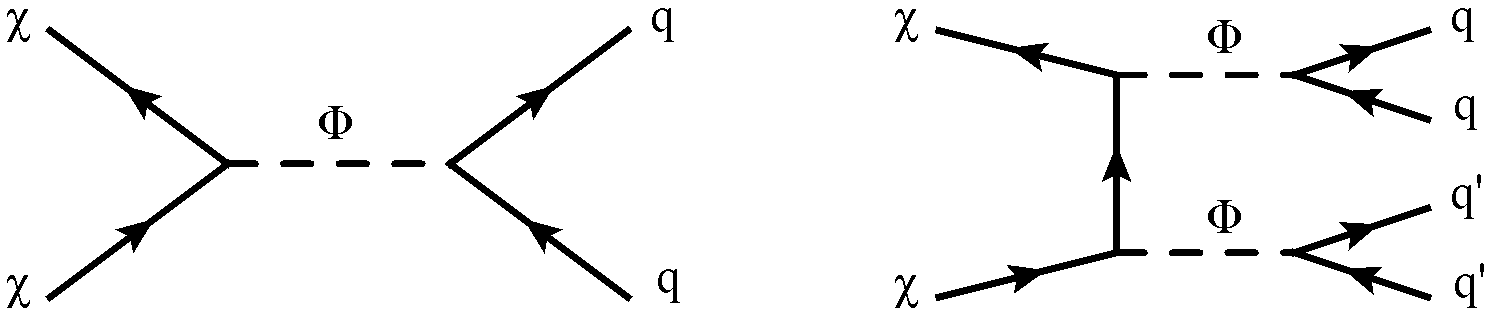
\includegraphics[width=0.78\textwidth]{figures/DMAnnihilationDiagrams.png} 
\vspace{4mm}
\caption{Feynman graphs of 
%G.B.: removed and changed %s-channel (left) and t-channel (right) DM annihilation. 
DM $s$-channel annihilation to quarks (left) and $t$-channel annihilation to a pair of mediators subsequently decaying to quarks (right). The exchanged~$\Phi$ particle(s) can be either (pseudo-)scalar or (axial-)vector mediator(s). %While the $s$-channel process is dominant for $M_{\rm med}/2 \geq m_{\rm DM}$, the region $M_{\rm med} \leq m_{\rm DM}$ is dominated by the $t$-channel diagram.
}
\label{fig:relicprod}
\end{figure}
\end{center}

Analytic %Uli forms
expressions 
% 
for the annihilation cross sections can be derived separately for both %Uli processes 
Feynman diagrams 
% 
in Figure~\ref{fig:relicprod}. 
In the case of the $s$-channel graphs we obtain 
\begin{align}
\sigma_{{\rm ann},s}^S \cdot v & = \sum_{q} \frac{N_c^q \hspace{0.125mm} g_{\rm DM}^2  \hspace{0.5mm} y_q^2 \hspace{0.25mm} g_q^2 \hspace{0.5mm}  \beta_q}{16 \pi}  \, \frac{m_{\rm DM}^2 - m_q^2}{\left (M_{\rm med}^2 - 4 m_{\rm DM}^2 \right )^2 + M_{\rm med}^2 \Gamma_{\rm med}^2} \; v^2 \,, \label{eq31} \\
\sigma_{{\rm ann},s}^P \cdot v & = \sum_{q} \frac{N_c^q \hspace{0.125mm} g_{\rm DM}^2 \hspace{0.5mm} y_q^2 \hspace{0.25mm} g_q^2  \hspace{0.5mm} \beta_q}{4 \pi}  \, \frac{m_{\rm DM}^2}{\left (M_{\rm med}^2 - 4 m_{\rm DM}^2 \right )^2 + M_{\rm med}^2 \Gamma_{\rm med}^2} \,, \label{eq32} \\
\sigma_{{\rm ann},s}^V \cdot v & = \sum_{q} \frac{N_c^q \hspace{0.125mm} g_{\rm DM}^2 \hspace{0.25mm} g_q^2 \hspace{0.5mm} \beta_q}{2 \pi} \,  \frac{2 m_{\rm DM}^2+ m_q^2}{\left (M_{\rm med}^2 - 4 m_{\rm DM}^2 \right )^2 + M_{\rm med}^2 \Gamma_{\rm med}^2} \,, \label{eq33} \\
\sigma_{{\rm ann},s}^A \cdot v & = \sum_{q} \frac{N_c^q \hspace{0.125mm} g_{\rm DM}^2 \hspace{0.25mm} g_q^2  \hspace{0.5mm} \beta_q}{2 \pi}  \frac{ m_{q}^2 \left ( 4 m_{\rm DM}^2- M_{\rm med}^2  \right)^2}{M_{\rm Med}^4 \left [ \left (M_{\rm med}^2 - 4 m_{\rm DM}^2 \right )^2 + M_{\rm med}^2 \Gamma_{\rm med}^2 \right ] } \,, \label{eq34}
\end{align}
where the sum includes all quarks with $m_q \leq m_{\rm DM}$, $N_c^q =3$, $\beta_q = \sqrt{1 - m_q^2/m_{\rm DM}^2}$ and~$v$ is the 
relative velocity of the DM pair. Notice that in the pseudo-scalar, vector, and axial-vector case the $s$-channel annihilation cross section proceeds via $s$-wave,~i.e.~it is of ${\cal O} (v^0)$, while in the case of scalar exchanges DM annihilation is $p$-wave suppressed,~i.e.~it is of ${\cal O} (v^2)$. The corresponding annihilation cross sections into charged leptons can be obtained from the above expressions by a suitable replacement of color factors and SM fermion masses. 

In the case of the $t$-channel diagrams we instead find  the following annihilation cross sections
\begin{align}
\sigma_{{\rm ann},t}^S \cdot v & =  \frac{ g_{\rm DM}^4   \hspace{0.5mm} \beta_{\rm med}}{24 \pi}  \, \frac{ m_{\rm DM}^2 \left ( 9 m_{\rm DM}^4  - 8 m_{\rm DM}^2 M_{\rm med}^2  + 2 M_{\rm med}^4   \right )}{\left (M_{\rm med}^2 - 2 m_{\rm DM}^2 \right )^4}  \; v^2 \,, \label{eq35} \\
\sigma_{{\rm ann},t}^P \cdot v & =  \frac{ g_{\rm DM}^4   \hspace{0.5mm} \beta_{\rm med}}{24 \pi} \,  \frac{m_{\rm DM}^2 \left (  m_{\rm DM}^2  - M_{\rm Med}^2  \right )^2}{\left (M_{\rm med}^2 - 2 m_{\rm DM}^2 \right )^4}  \; v^2 \,, \label{eq36} \\
\sigma_{{\rm ann},t}^V \cdot v & =  \frac{ g_{\rm DM}^4   \hspace{0.5mm} \beta_{\rm med}}{4 \pi}  \, \frac{m_{\rm DM}^2 - M_{\rm med}^2 }{\left (M_{\rm med}^2 - 2 m_{\rm DM}^2 \right )^2}  \,, \label{eq37} \\
\sigma_{{\rm ann},t}^A \cdot v & =  \frac{ g_{\rm DM}^4   \hspace{0.5mm} \beta_{\rm med}}{4 \pi}  \, \frac{m_{\rm DM}^2 - M_{\rm med}^2  }{\left (M_{\rm med}^2 - 2 m_{\rm DM}^2 \right )^2} \,, \label{eq38}
\end{align}
for $M_{\rm med} \leq m_{\rm DM}$. Here $\beta_{\rm med} = \sqrt{1-M_{\rm med}^2/m_{\rm DM}^2}$ and one observes that the  annihilation of DM into a pair of mediators is $p$-wave ($s$-wave) in the case of spin-0 (spin-1) exchanges. From the above results it follows that in the case of scalar, vector, and axial-vector interactions both $s$-channel and $t$-channel annihilation has to be considered, while in the case of a pseudo-scalar typically only the $s$-channel contribution is relevant. We add that in some of the cases with non-vanishing $s$-wave contribution the $p$-wave contribution is nevertheless numerically relevant. This is for instance the case for  the axial-vector mediator where the $s$-wave contribution to the $s$-channel is helicity suppressed, while the $t$-channel receives only contributions from longitudinal polarizations. We do not provide the corresponding expressions here but included them in the numerical results presented below.

Using the velocity expansion\footnote{This expansion breaks down close to an $s$-channel resonance, 
making a numerical solution indispensable.}  $\sigma_{\rm ann} \cdot v = a + b v^2 + {\cal O} (v^4)$ the DM relic density  after freeze-out is approximately given by
\begin{equation}
    \Omega h^2 \simeq 0.12 \; \frac{1.6 \cdot 10^{-10} \, x_f \, {\rm GeV}^2}{a + \frac{3b}{x_f}} \,,
\end{equation}
where $x_f = m_{\rm DM}/T_f$ with $T_f$ the freeze-out temperature. In our comparison between analytic and numerical results we will employ $x_f = 28$. For this value of $x_f$ the correct relic abundance thus occurs in the ballpark of
\begin{equation}
2.2 \cdot 10^{-26} \, {\rm cm}^3/{\rm s} \simeq 4.5 \cdot 10^{-9} \, {\rm GeV}^{-2} \simeq a + 0.1 \hspace{0.25mm} b \,.
\end{equation}

%
%\begin{equation}
%\label{eq:SS}
%    \Omega h^{2}  \propto  \left[\Sigma_{q} \frac{g_{\rm DM}^2 g_{\rm q}^2 y_{q}^2}{32\pi s } %\frac{\left(s-4m^2_{q}\right)^{3/2}\sqrt{s-4m_{\rm DM}^2}}{\left(s-m_{\rm med}^2\right)^2} \right]^{-1} \
%\end{equation}
%\begin{equation}
%\label{eq:SV}
%\Omega h^{2} & \propto & \left[\Sigma_{q} \frac{g_{\rm DM}^2 g_{\rm q}^2           }{32\pi s } %\frac{\left(s-4m^2_{q}\right)^{3/2}        (s+2m_{\rm DM}^2)}{\left(s-m_{\rm med}^2\right)^2\sqrt{s-4m_{\rm DM}^2}} \right]^{-1}
%\end{equation}
%
%\begin{eqnarray}
%\label{eq:SS} \Omega h^{2}_{S} & \propto & \left[\sum_{q} \frac{g_{\rm DM}^2 g_{q}^2 y_{q}^2}{32\pi s } \frac{\left(s-4m^2_{q}\right)^{3/2}\sqrt{s-4m_{\rm DM}^2}}{\left(s-m_{\rm med}^2\right)^2} \right]^{-1} \,, \\
%\label{eq:SV} \Omega h^{2} & \propto & \left[\Sigma_{q} \frac{g_{\rm DM}^2 g_{\rm q}^2           }{32\pi s } \frac{\left(s-4m^2_{q}\right)^{3/2}        (s+2m_{\rm DM}^2)}{\left(s-m_{\rm med}^2\right)^2\sqrt{s-4m_{\rm DM}^2}} \right]^{-1}. %This was the vector (not axial) equation
%\label{eq:SV} \Omega h^{2}_{V} & \propto & \Bigg[ \sum_q \frac{\beta_q }{16 \pi \beta_{\rm DM}} \frac{  (g_q g_{\rm DM})^2 s }{(s-m_{\rm med}^2)^2 +m_{\rm med}^2\Gamma_{\rm med}^2 }\times \Big(3+\beta_{\rm DM}^2 \beta_q^2 
%\nonumber\\
%		 && \phantom{x} -12\frac{m_{\rm DM}^2}{s}-12\frac{m_q^2}{s}
%		 +96 \frac{m_q^2 m_{\rm DM}^2}{s^2} -96 \frac{m_q^2 m_{\rm DM}^2}{s m_{\rm med}^2}
%		 +48 \frac{m_q^2 m_{\rm DM}^2}{m_{\rm med}^4} \Big) \Bigg]^{-1} \,,
%\end{eqnarray}
%where $\beta_q = \sqrt{1-4m_q^2/s}$ and $\beta_{\rm DM} = \sqrt{1-4m_{\rm DM}^2/s}$. The summation over $q$ includes all quark flavour for which $m_{q} < m_{\rm DM}$, while $y_{q} = \sqrt{2} m_q/v$ with $v \simeq 246 \, {\rm GeV}$ denotes the SM Yukawa couplings. The masses of mediator and DM particle are denoted by $m_{\rm med}$ and $m_{\rm DM}$, respectively. Finally, $s$ denotes the center of mass energy, which varies as the Universe cools. {\bf [Uli: $s$ can be expanded in the laboratory frame as $s = 4 m_{\rm DM}^2 + m_{\rm DM}^2 v^2 + {\cal O} (v^4)$ with $v \simeq 10^{-3} c$ the DM velocity. I would suggest to insert this expansion into (3.1) and (3.2) and to determine and to give only the leading terms in $v$. One should also briefly comment on the pseudo-scalar and axial-vector cases. That the mediator width is included in (3.2) but not in (3.1) looks also a bit strange.]}   


%CD: removed, what does this mean?
%In this analytic expression, the reciprocal relationship between the relic density and coupling parameters is evident. 
%\textbf{[Mention leptons?]} {\bf [Uli: I would simply say that leptons are not relevant for the discussion. BTW, are they included in the numerical analysis?]}

%Similarly, one can derive the relic density expression
%CD: not sure closed form is something that we want to use here?
%a closed form 
%for the t-channel process, where~\ref{eq:TS} represents the scalar and~\ref{eq:TV} the axial-vector scenario:

%The $t$-channel contributions to the relic density are given in the scalar and axial-vector case by 
%\begin{equation}
%\label{eq:TS}
%\Omega h^2  \propto  \left g_{\rm DM}^4\frac{m_{\rm DM}\sqrt{m_{\rm DM}^2-m_{\rm med}^2}( 9m_{\rm DM}^4+8m_{\rm DM}^2m_{\rm med}^2+2m_{\rm med}^4)}{3\pi\left(m_{\rm med}^2-2m_{\rm DM}^2\right)^4} \right]^{-1}
%\end{equation}
%
%\begin{equation}
%\label{eq:TV}
%\Omega h^2  \propto  FORMULA 
%\end{equation}
%
%\begin{eqnarray}
%\label{eq:TS} \Omega h^2_{S} & \propto & \left[g_{\rm DM}^4\frac{m_{\rm DM}\sqrt{m_{\rm DM}^2-m_{\rm med}^2}( 9m_{\rm DM}^4+8m_{\rm DM}^2m_{\rm med}^2+2m_{\rm med}^4)}{3\pi\left(m_{\rm med}^2-2m_{\rm DM}^2\right)^4} \right]^{-1} \,, \\  
%\label{eq:TV} \Omega h^2_{A} & \propto & \left[\frac{ (g_{\rm DM})^4 (m_{\rm DM}^2 - m_{\rm med}^2)^{3/2}}{4 \pi \, m_{\rm DM}(m_{\rm med}^2 - 2 m_{\rm DM}^2)^2}  \right]^{-1}   \,.  
%\end{eqnarray}
%{\bf OB: Need to add formula for~\label{eq:TV}}
%PT: I have added this formula. It is correct under the assumptions I've added towards the end
%{\bf [Uli: What about the pseudo-scalar and axial-vector cases. I guess they must be velocity suppressed, but saying this explicitly would help. Again I would suggest to expand (3.3) and (3.4) in $v$.]}

\subsection{Numerical results}
\label{numericrelic}

One can improve upon the analytic calculation described above by performing a numerical calculation %Uli of a larger set of processes 
that also takes into account the thermal evolution of the Universe. The results presented in this subsection rely on \maddm version 2.0.6.  The \maddm package considers all tree-level $2\rightarrow2$ interactions between DM and SM particles. The processes are thermally averaged and the resulting relic density is computed.
Since \maddm does not yet automatically calculate the mediator width from the model parameters, the \dmsimp model was modified to use the mediator width formulas presented for instance in~\cite{Abercrombie:2015wmb,Boveia:2016mrp}. % \cite{Abercrombie:2015wmb,DarkMatterWidthCalculator,Boveia:2016mrp}. 
The DM density calculations provided in the previous LHC DM WG recommendations~\cite{Boveia:2016mrp} %\cite{Boveia:2016mrp,Pree:2016hwc} 
used an earlier version of \maddm which did not include  $t$-channel annihilation to pairs of mediators. Below we will comment on the effects that this omission has.  

%ABCD: Below not significant because they've been tested 
%Less significantly, since the \dmsimp implementation was not available at the time, the results were derived using a previous implementation of  simplified models, which are however equivalent to the \dmsimp models in physics content.

\begin{center}
\begin{figure}[h]
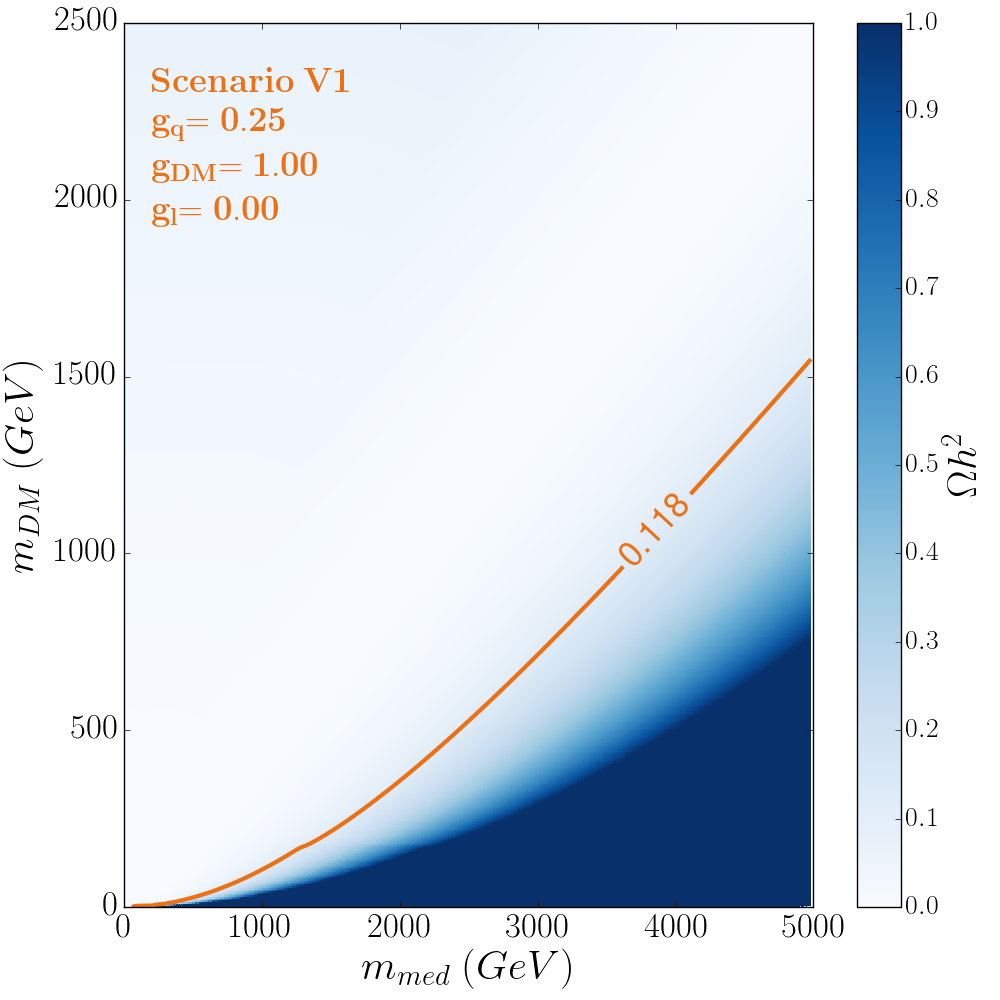
\includegraphics[width=0.49\textwidth]{figures/relic_V1.png} 
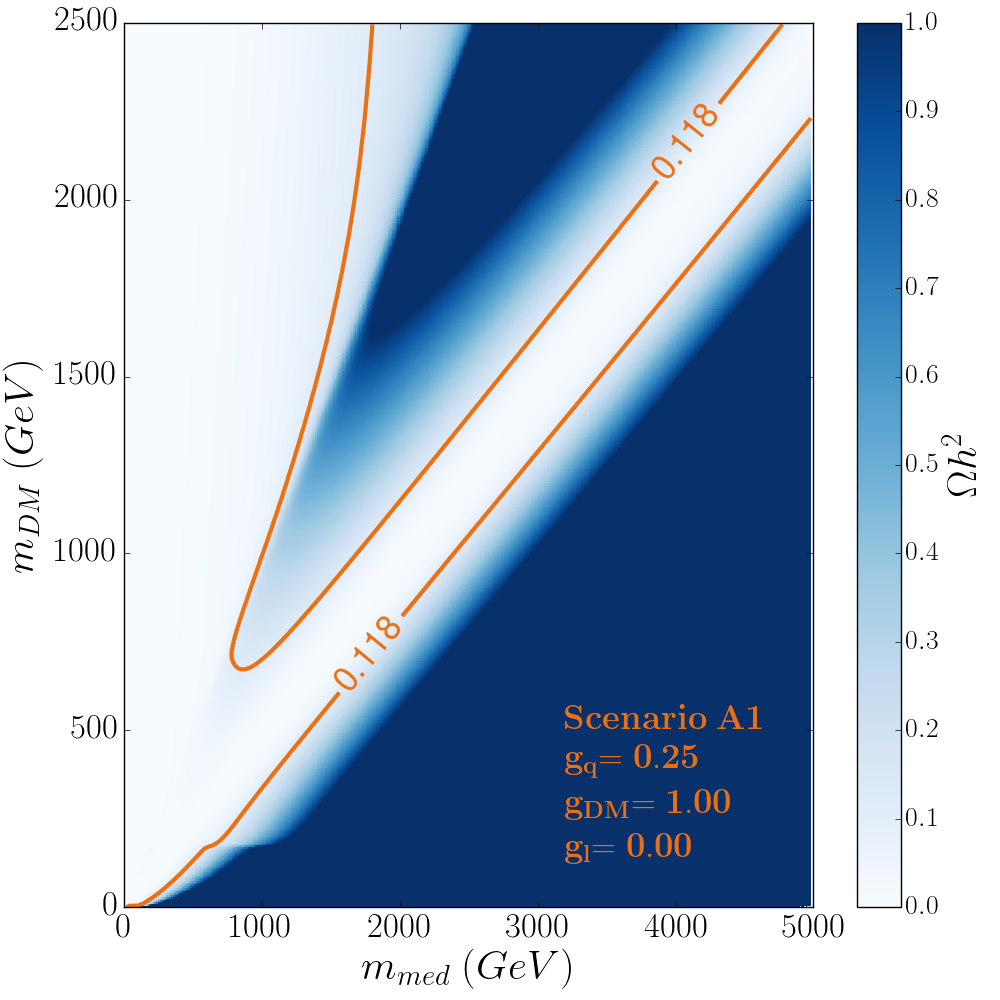
\includegraphics[width=0.49\textwidth]{figures/relic_A1.png} \\[2mm]
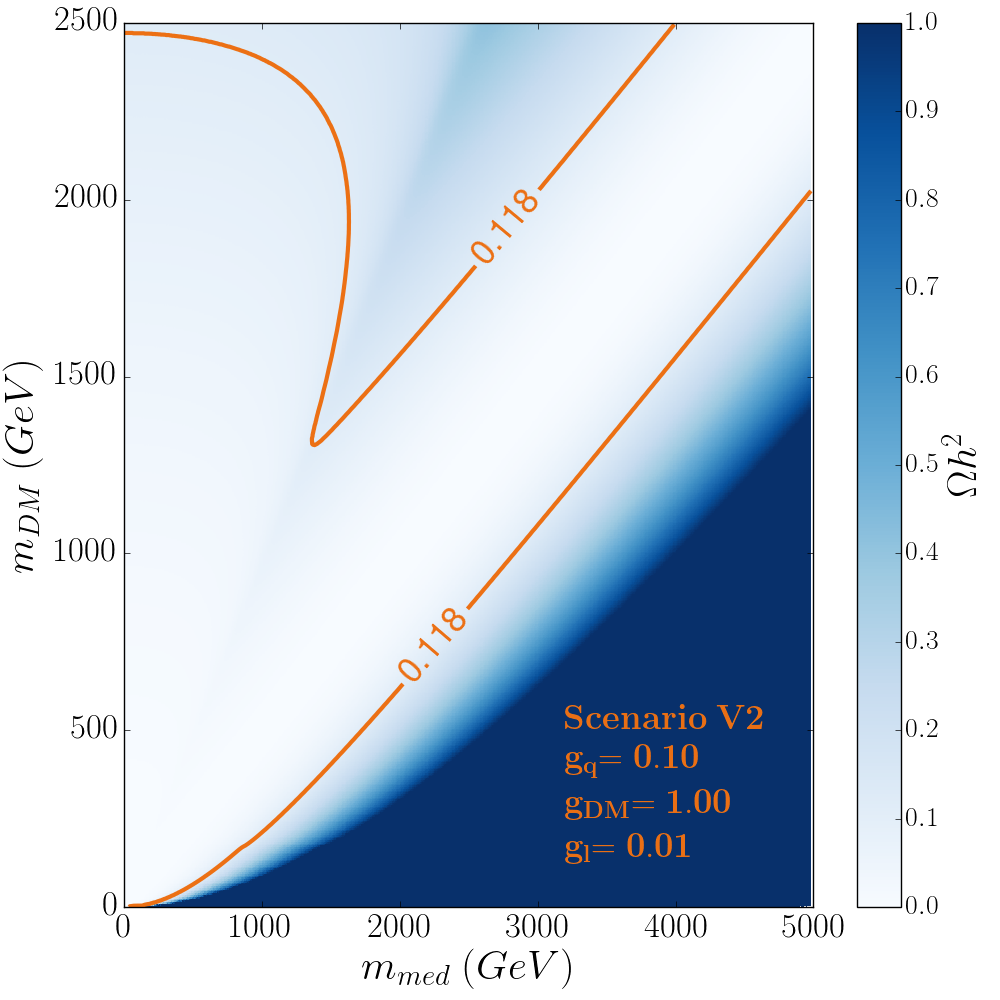
\includegraphics[width=0.49\textwidth]{figures/relic_V2.png} 
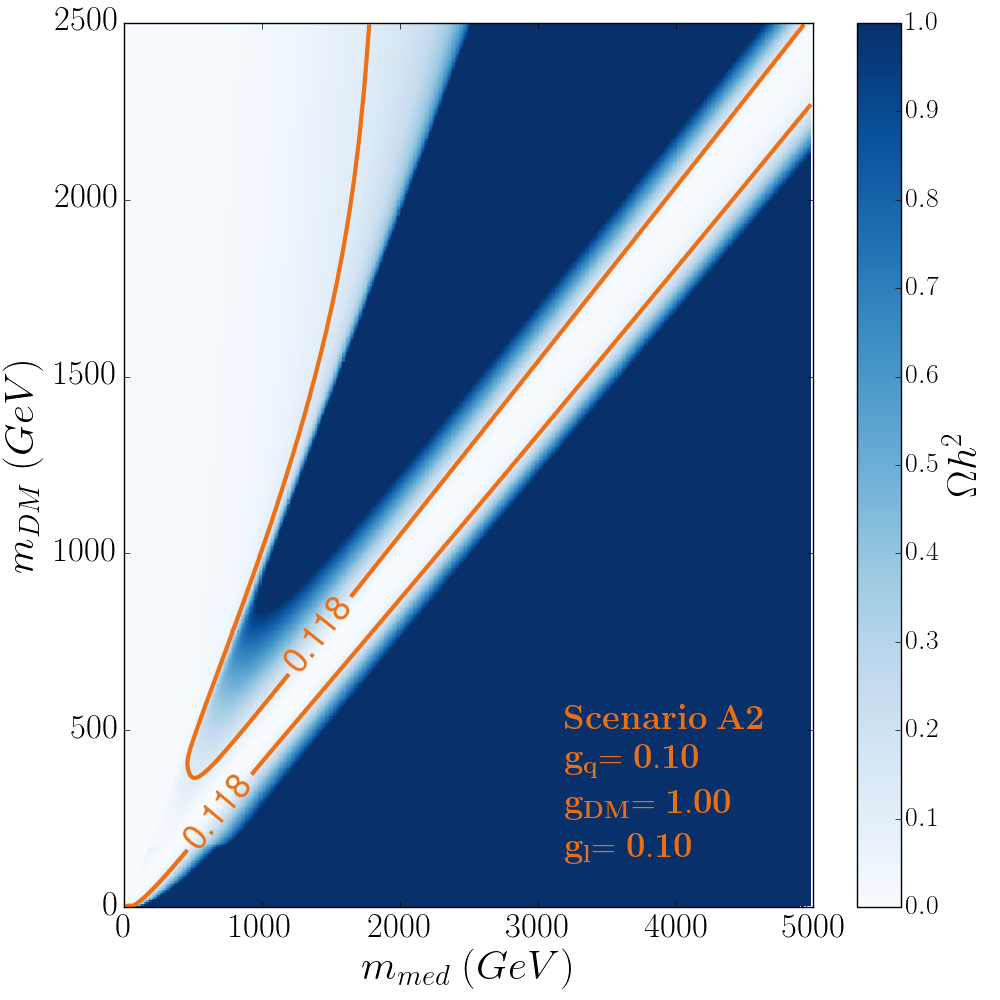
\includegraphics[width=0.49\textwidth]{figures/relic_A2.png} \\[-4mm]
\caption{The relic density $\Omega h^{2}$ in the $M_{\rm med}$--$m_{\rm DM}$ plane predicted by the four spin-1 scenarios  described in Section~\ref{sub:vecAxial}. All couplings to DM are set to unity ($g_{\rm DM}=1.0$). Top left: scenario V1, vector mediator with couplings only to quarks ($g_{ q}=0.25$). Top right:
scenario A1, axial-vector mediator with couplings only to quarks ($g_{q}=0.25$). 
 Bottom left: scenario V2, vector mediator with couplings to quarks and small couplings to leptons ($g_{ q}=0.1$ and $g_{\ell}=0.01$). Bottom right: scenario A2, axial-vector mediator with equal couplings to quarks and leptons ($g_{q}=0.1$ and $g_{\ell}=0.1$).
The contour lines correspond to the region of parameter space where the relic density is consistent with the value $\Omega h^2=0.118$. %Uli  The impact of the uncertainty on the position of the contours is consistent with the line width.
}
\label{fig:DMBoundsScenarios}
\end{figure}
\end{center}

The panels in Figures~\ref{fig:DMBoundsScenarios} and \ref{fig:DMBoundScalars} show the predictions for the relic density $\Omega h^2$ in the $M_{\rm med}$--$m_{\rm DM}$ plane for spin-1 and spin-0 mediators, respectively. In the spin-1 case the  coupling scenarios described in Section~\ref{sub:vecAxial} are employed, while for the spin-0 models the standard coupling values $g_{\rm DM} = g_q =1$ and $g_{\ell} = 0$ have been used. The solid contours in all panels indicate the combination of masses for which the correct DM abundance $\Omega h^2 = 0.118$~\cite{Ade:2015xua} is obtained. The parts in the  $M_{\rm med}$--$m_{\rm DM}$ plane where the relic density is either higher or lower than the observed value are referred to as overabundant and underabundant regions, respectively.

One observes that all models predict an overabundance of DM for $M_{\rm med} \gg m_{\rm DM}$. While the shape and exact size of this region depend on the specific model realisation, larger quark couplings $g_{q}$ in general allow DM to annihilate into SM particles more efficiently, which reduces the parameter space over which overabundance can occur.

For the vector  scenario V1 (top left panel in Figure \ref{fig:DMBoundsScenarios}) only a single overabundant region with $M_{\rm med} \gg m_{\rm DM}$ is present. For the shown part of the $M_{\rm med}$--$m_{\rm DM}$ plane this case is fully consistent with previous results (see e.g.~\cite{Boveia:2016mrp,Busoni:2014gta, Pree:2016hwc}). In the axial-vector scenario~A1~(top right panel in Figure \ref{fig:DMBoundsScenarios}) the  overabundance region extends to higher $m_{\rm DM}$ values than in scenario V1. Additionally, there is an overabundance region above the diagonal $m_{\rm DM}=M_{\rm med}/2$. While this region is also present in the corresponding figures  of~\cite{Pree:2016hwc} its width in mediator mass is significantly narrower. 
The observed difference is due to $t$-channel annihilation diagrams to pairs of mediators that have not been included in the latter work but are relevant if  $M_{\rm med}<m_{\rm DM}$. 

%Was: In both axial vector scenario A2 and pure vector scenario V2 ($g_{\rm q}=0.1$), the relic density is suppressed with respect to the corresponding scenarios A1 and V1 ($g_{\rm q}=0.25$) as a result of the increasing annihilation cross-section due to the decreasing quark couplings. This causes an overabundance region to appear in scenario V2. 

In both the vector scenario V2 and axial-vector scenario A2 (lower left and right plot in Figure~\ref{fig:DMBoundsScenarios}) the relic density is  %Uli I think it should say enhanced instead of suppressed 
enhanced with respect to the corresponding scenarios V1~and~A1. This is a result of the quark couplings being smaller in  V2 and~A2 than in V1 and~A1. Decreasing the quark couplings however reduces the annihilation cross section, which in turn  leads to an overabundance of DM for larger parts of the $M_{\rm med}$--$m_{\rm DM}$ plane. We add that for scenario V2 with  $g_{\ell} = 0.01$, DM annihilation into leptons has essentially no effect on $\Omega h^2$.  In scenario A2 with $g_{\ell} = 0.1$ the relic density is instead slightly suppressed in the whole $M_{\rm med}$--$m_{\rm DM}$ plane compared to a model with quark couplings only.  

\begin{center}
\begin{figure}[t!]
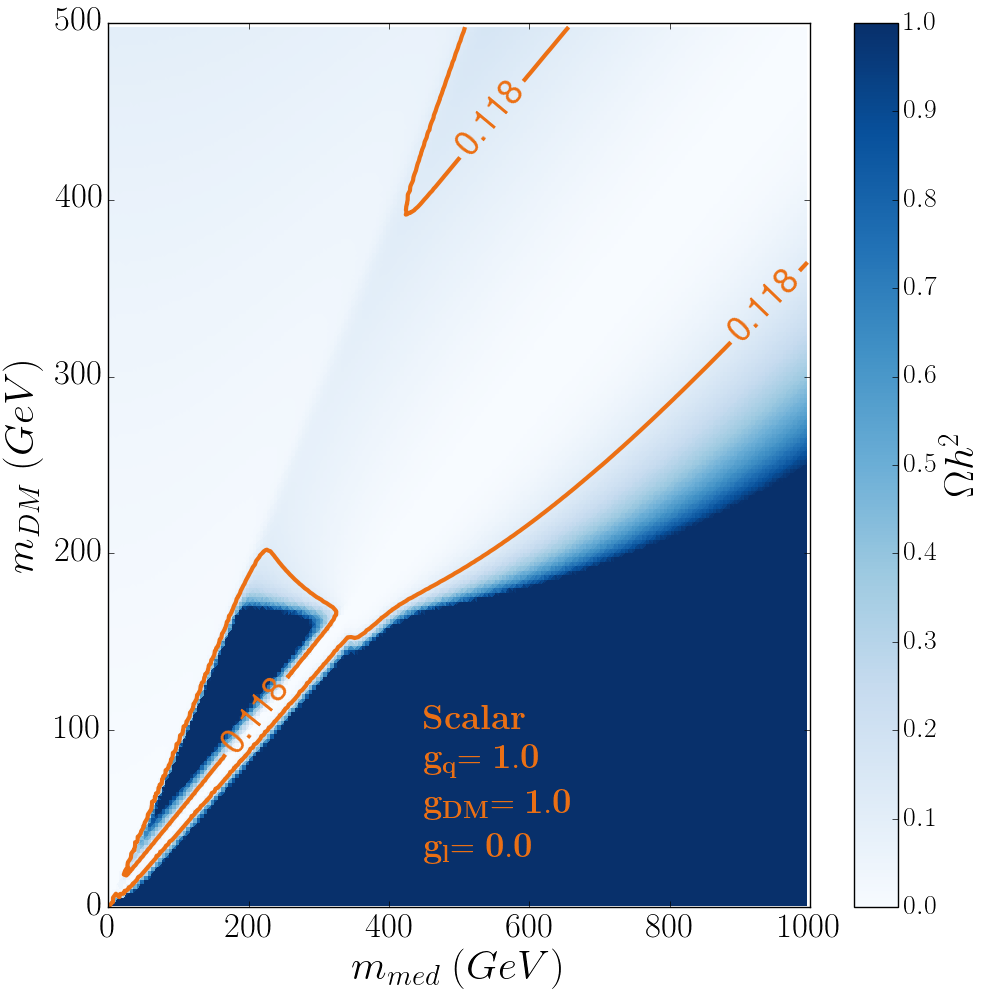
\includegraphics[width=0.49\textwidth]{figures/relic_scalar_gq1.png} 
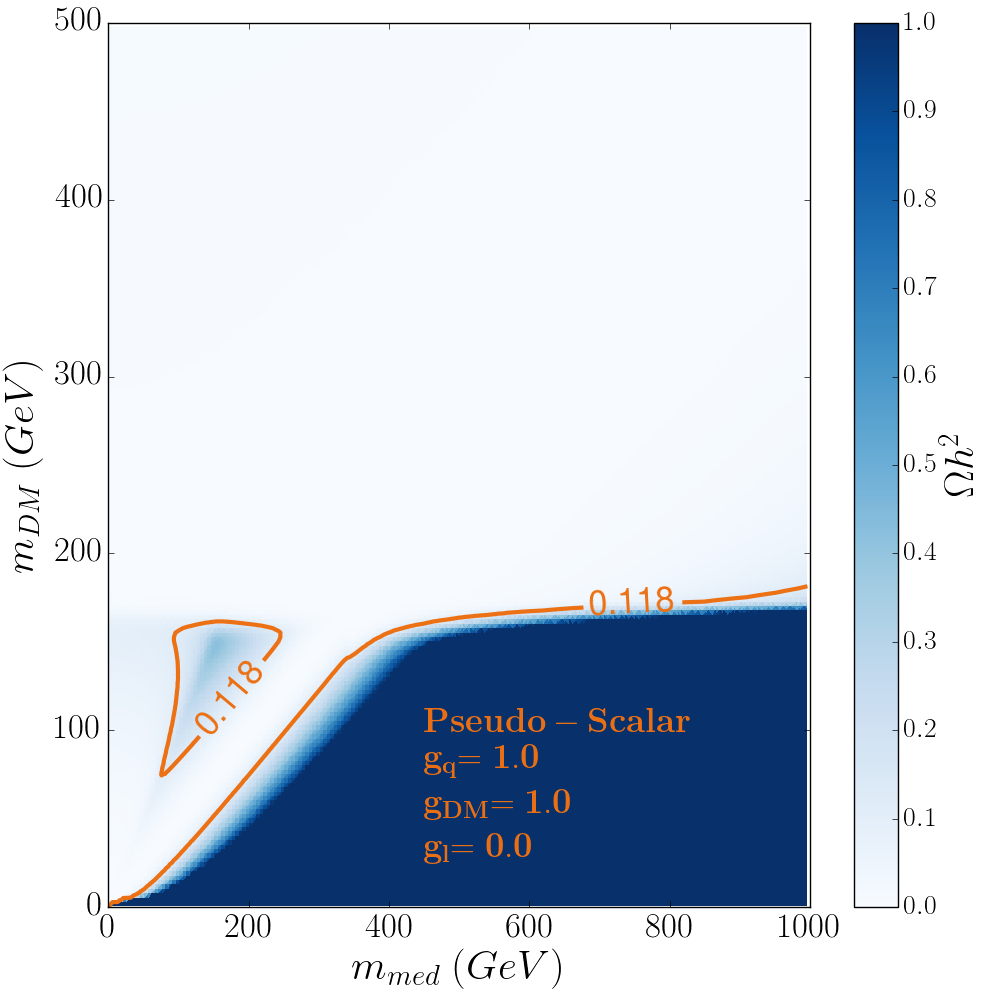
\includegraphics[width=0.49\textwidth]{figures/relic_pseudo_gq1.png} \\
\caption{The relic density $\Omega h^{2}$ in the $M_{\rm med}$--$m_{\rm DM}$ plane predicted by the scalar (left panel) and pseudo-scalar (right panel) mediator models with couplings $g_{\rm DM} = g_q =1.0$.
The contour lines indicate the observed value of the DM relic density $\Omega h^2=0.118$. }
\label{fig:DMBoundScalars}
\end{figure}
\end{center}

Notice finally that in the case of axial-vector mediation, $s$-channel annihilation proceeds via $s$-wave but is helicity suppressed, while for vector mediators no such suppression occurs $\big($cf.~(\ref{eq33}) and (\ref{eq34})$\big)$. This feature qualitatively explains why the regions with DM overabundance are typically larger for axial-vector scenarios than for vector models. 







%The order of magnitude of the change can be naively
%estimated by the change in the cross-section, which is ~25% near the
%resonance line Mmed = 2*mDM (this value changes across the plane). Since
%the contours are located on steep flanks of the 2D landscape, the
%density change only causes a small shift of the contours.






For the scalar simplified model (left panel in Figure~\ref{fig:DMBoundScalars}), the overabundance region for small $m_{\rm DM}$ is fades out for $m_{\rm DM}$ values above the top threshold $m_t$, above which annihilation of DM pairs into top-quark pairs is allowed. Additional overabundance regions occur for $M_{\rm med} > m_{\rm DM} > M_{\rm med}/2$, where the upper bound is due to the onset of mediator pair production and the lower bound reflects the resonant enhancement of DM annihilation to SM particle pairs. A region of overabundance at $M_{\rm med} > m_{\rm DM}$ in the predictions shown in~\cite{Pree:2016hwc} is now underabundant after including the $t$-channel annihilation contributions.

The pseudo-scalar simplified model (right panel in Figure~\ref{fig:DMBoundScalars}) is similar to the scalar scenario, with less pronounced regions of overabundance due to the increased annihilation cross section from $s$-channel $s$-wave contributions. Consequently, no regions of overabundance are observed above the top threshold and the triangular region present for the scalar model at $M_{\rm med}/2 < m_{\rm DM}$ is reduced in size compared to~\cite{Pree:2016hwc}. 

\subsection{Comparison of analytic results to full numerical calculations}

\begin{center}
\begin{figure}[t!]
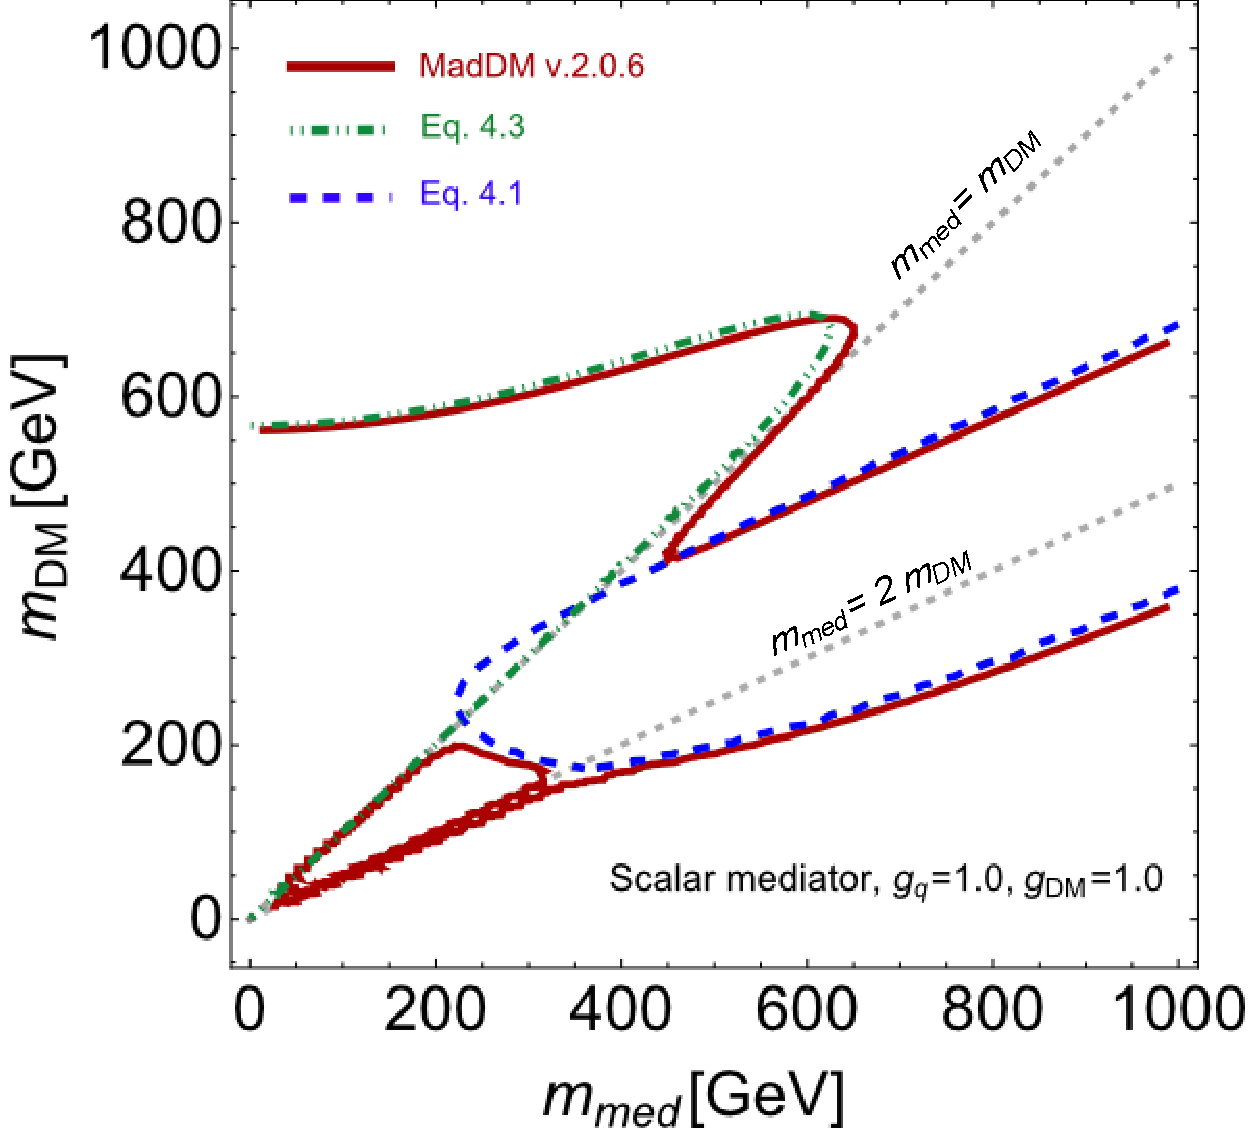
\includegraphics[width=0.49\textwidth]{figures/scalar_mediator_omegah2.pdf}
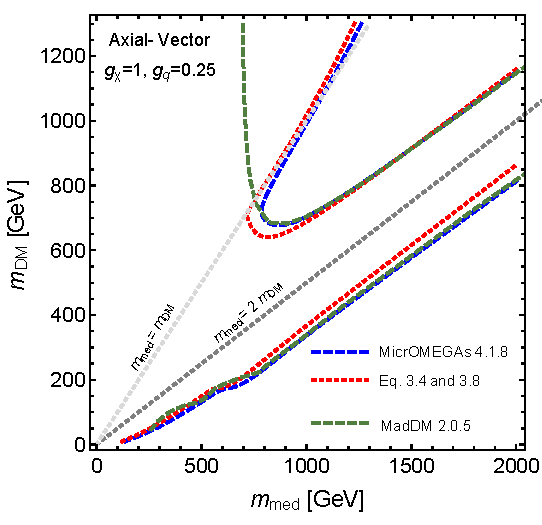
\includegraphics[width=0.47\textwidth]{figures/AV_comparison2.pdf} 
\caption{Comparison of the analytic calculations described in Section~\ref{analyticrelic}  with numerical results obtained with \maddm and \textsc{MicrOMEGAs}. In the scalar case (left panel) the exact numerical results have been obtained with version 2.0.6 of \maddm, while for the axial-vector mediator model (right panel)
version 4.1.8 of \textsc{MicrOMEGAs} has been used to calculate the relic density. See main text for further details.}
\label{fig:analcalc}
\end{figure}
\end{center}

In Figure~\ref{fig:analcalc} we compare the results of the analytic calculations described in Section~\ref{analyticrelic}  with full numerical results obtained with the packages \maddm and \textsc{MicrOMEGAs}~\cite{Belanger:2014vza}. The left~(right) panel shows the contours in the $M_{\rm med}$--$m_{\rm DM}$ plane for which $\Omega h^2 = 0.118$ in the case of scalar (axial-vector) interactions for the coupling choices $g_{\rm DM} = 1$ and $g_q = 1$~($g_q = 0.25$). The analytic results are obtained by employing~(\ref{eq31}) and (\ref{eq35}) in the case of the scalar mediator, while (\ref{eq34}) and (\ref{eq38}) are used for the axial-vector simplified model. In both cases the ratio of the DM mass to freeze-out temperature is fixed to~$x_f = 28$ and also the effective number of relativistic degrees of freedom is kept constant across the~$M_{\rm med}$--$m_{\rm DM}$ plane.

From both panels it is evident that in the limiting cases where one of the channels dominates the annihilation cross sections, the analytic calculations are in good agreement with the numerical results obtained either by version 2.0.6 of \maddm (scalar case) or version 4.1.8 of \textsc{MicrOMEGAs} (axial-vector case). We emphasize that an improved agreement between analytic and numerical calculations can be obtained when using thermally-averaged cross sections and a numerically determined freeze-out temperature~\cite{Gondolo:1990dk}. In the case of the axial-vector model, we also display the contour line with $\Omega h^2 = 0.118$ using version 2.0.5 of \maddm. This prediction is used as representative of the results of \cite{Pree:2016hwc} that did not incorporate $t$-channel annihilation contributions. One observes that not taking into account the annihilation  contribution (\ref{eq38}) leads to an erroneous prediction of overabundance for $M_{\rm med} < m_{\rm DM}$. We have also verified that version 2.0.6 of \maddm and version 4.1.8 of \textsc{MicrOMEGAs} lead to compatible result for axial-vector simplified models. 


%CD: too much detail for this paper? For now footnoted. 
%The analytic results in Fig.~\ref{fig:analcalc} are based on an estimate of the ratio of the DM mass to freeze-out temperature. For the axial vector, we assumed this ratio to be 28 across the parameter space, and similarly estimated the effective number of relativistic degrees of freedom. We expanded the cross section in powers of the DM velocity which is not exact and care should be taken with this approach since it can break down in certain regimes, for example on resonance~\cite{Gondolo:1990dk}.




